\documentclass[12pt,spanish,letterpaper]{article}
\usepackage[spanish,activeacute]{babel}
\usepackage[utf8]{inputenc}
\usepackage{amsthm,amsfonts,amsmath,fancyhdr,dsfont,hyperref,amssymb,multicol,graphicx,float,booktabs,arydshln,hhline,colortbl}
%% SWAP THE COMMENT IN THE FOLOWING LINES TO USE COLOR BORDERS IN TABLES
%\usepackage[usenames,dvipsnames]{color}
\usepackage{xcolor}
\newtheorem{teo}{Teorema}[section]
\newtheorem{cor}{Corolario}[section]
\newtheorem{lem}{Lema}[section]
\newtheorem{defi}{Definición}[section]
\newtheorem{prop}{Proposición}[section]
\pagestyle{fancy}
\fancyhead[LE,LO]{\footnotesize{\sc{Pablo Estefó Carrasco}}} %Header Left
\fancyhead[CE,CO]{\footnotesize{\sc{}}} %Header Center
\fancyhead[RE,RO]{\footnotesize{\sc{CC6908 - Introducción al Trabajo de Título}}} %Header Right
\fancyfoot[LE,LO]{\footnotesize{}} %Footer Left
\fancyfoot[CE,CO]{\footnotesize{\thepage}} %Footer Center
\fancyfoot[RE,RO]{\footnotesize{}} %Footer Right
\headwidth 6.5in
\hoffset 0in
\voffset 0in
\oddsidemargin 0in
\marginparwidth 0in
\marginparsep 0in
\headsep 0.15in
\topmargin 0in
\textwidth 6.5in
\textheight 8.5in
%Comandos para mostrar correctamente las demostraciones
\newcommand{\halmos}{\rule{2mm}{2mm}}
\renewcommand{\qedsymbol}{\halmos}
%Comandos definidos míos
\newcommand\VRule[1][\arrayrulewidth]{\vrule width #1}
\newcommand{\paren}[1]{\left(#1\right)}
\newcommand{\parencuad}[1]{\left[#1\right]}
\newcommand{\parenllav}[1]{\left\{#1\right\}}
\newcommand{\deriv}[2]{\frac{d #1}{d #2}}
\newcommand{\derivpar}[2]{\frac{\partial #1}{\partial #2}}
\newcommand{\overarc}[1]{\stackrel \frown {#1}}
\thispagestyle{empty}
\begin{document}
\thispagestyle{empty}
\begin{minipage}{\textwidth}
	Universidad de Chile\\
	Facultad de Ciencias Físicas y Matemáticas\\
	Departamento de Ciencias de la Computación\\
	CC6908 - Introducción al Trabajo de Título
\end{minipage}
\vfill
\begin{minipage}{\textwidth}
	\begin{center}
		\huge{Reestructuración y Refactorización de Unit Tests con TestSurgeon}
	\end{center}
\end{minipage}
\vfill
\begin{minipage}{\textwidth}
	\begin{tabular}{c}
		\hline
		Alexandre Bergel\\
		abergel@dcc.uchile.cl\\
		Profesor Guía
	\end{tabular}
	\hfill
	\begin{tabular}{c}
		\hline
		Pablo Estefó Carrasco\\
		paestefo@dcc.uchile.cl\\
		Alumno
	\end{tabular}
	\vspace{1.5cm}
\end{minipage}
\begin{minipage}{\textwidth}
	\null
	\hfill
	\begin{minipage}{3.25in}
		\begin{tabular}{rl}
			Nombre:&Pablo Ignacio\\
			&Estefó Carrasco\\
			Correo:&paestefo@dcc.uchile.cl\\
			Teléfono:&(02) 8131062\\
			Móvil:&(09) 83409945\\
			Fecha:&10 de diciembre de 2012
		\end{tabular}
	\end{minipage}
\end{minipage}
\newpage
\pagenumbering{roman}
\tableofcontents
\newpage
\pagenumbering{arabic}

%%%%%%%%%%%%%%%%%%%%%%%%%%%%%%%%%%%%%%%%%%%%%
% MOTIVACION
%%%%%%%%%%%%%%%%%%%%%%%%%%%%%%%%%%%%%%%%%%%%%

\section{Motivación}
\subsection{Contexto: Test como ``conductores'' del diseño}
\par Durante el desarrollo de un software uno de las actividades principales es el testeo de los requerimientos. Existen variadas técnicas, metodologías y artefactos relacionados a esta actividad. En particular, la creación de pruebas automatizadas es una práctica cotidiana en cualquier proyecto de software e inclusive es actualmente considerado parte de los artefactos generados durante éste. \\

\par En particular las metodologías ágiles dan una importancia fundamental a los tests de tal manera que está prohibido agregar una nueva funcionalidad sin, previamente, haber escrito un test que lo valide[\ref{tdd-beck}]. Esta queda documentado en el libro de Robert Cecil Martin (más conocido como``Uncle Bob'')[\ref{unclebob}] uno de los escritores del manifiesto ágil[\ref{agilemanifiesto}] quien declara:

\begin{quote}
\emph{``The iteration between writing test cases and code is very rapid [...]. As a result, a very complete body of test cases grows along with the code.''}
\end{quote}

\par Uno de los ejemplos más conocidos de implementación de estos principios es la metodología de Desarrollo Dirigido por Pruebas o \emph{Test-Driven Development}[\ref{tdd-beck}] el cual propone que la implementación de una funcionalidad del software debiera seguir los siguientes pasos:\\

\begin{enumerate}
\item Escribir un test que valide el funcionamiento esperado de la nueva característica
\item Escribir código base mínimo que haga pasar dicho test
\item Refactorizar el código
\end{enumerate}

\par En la práctica, aplicando TDD se obtiene una gran cantidad de pruebas unitarias (unit tests) que representan los casos de prueba de la aplicación (Test Cases). Cada Unit Test contiene varios métodos de tests (test methods) que cubren los distintos aspectos a verificar en la funcionalidad que se está testeando.

\subsection{Problema: Muchos tests, mal diseñados y lentos.}

\par La comunidad de ingeniería de software ha producido herramientas efectivas y buenas prácticas para lograr refactorizaciones en el código base que otorguen un buen diseño de código. Sin embargo, en cuanto al código de los tests unitarios no es así. De hecho, estos son raramente modificados y carecen del cuidado que se le da al código base y no se piensa en su modularidad ni extensibilidad. 

% ACTUALMENTE SOLO LES IMPORTA EL COVERAGE
\par Por lo cual no es difícil encontrar deficiencias como \textbf{solapamientos} entre test methods o más general, entre test cases. Estos solapamientos pueden ser de carácter estático: duplicación de código, o bien dinámicos, es decir que dos tests methods tienen ejecuciones similares y por consiguiente testean lo mismo. 
\par Estas deficiencias en el diseño y calidad del código de las pruebas unitarias tiene consecuencias importantes en la calidad del código testeado y en el mismo proceso de desarrollo:
\begin{itemize}
\item \textbf{Performance} Debido a los solapamientos previamente mencionados, muchas veces existe \textbf{ejecución redundante} que va en contra de las características deseables de una suite de tests[\ref{tdd-beck}]. Muchas veces los tests dejan de ejecutarse con la frecuencia deseada.
\item \textbf{Debugging} Otra deficiencia conocida es cuando al correr los tests en presencia de un defecto, éste se queda en evidencia por muchos tests methods, lo cual dificulta la identificación de la causa del bug y su corrección. Coloquialmente se hace más difícil responder la pregunta: \emph{¿Cuál test miro primero?}
\end{itemize}
 
\par De esta manera la confiabilidad en el producto y su calidad se ven impactadas negativamente. 

\par Un caso muy claro del impacto del mal diseño y poco cuidado en los tests sucede en la práctica de \textbf{Integración Contínua} (Continuous Integration)[\ref{contint}]. En esta práctica cada \emph{feature} se implementa tan pronto como es posible, se testea y se pasa a producción de inmediato. De esta manera el equipo de desarrollo realiza varias integraciones por día y el cliente obtiene rápidamente las nuevas funcionalidades a medida que las solicita. \\

\par A modo de ejemplo, la empresa MediaGeniX\footnote{MediaGeniX, \url{http://www.mediagenix.tv}} realiza la integración continua desde hace un tiempo. Ahí, 30 desarrolladores trabajan sobre el mismo producto y cada uno de ellos construye varias versiones al día. Cada versión que se va a pasar a producción debe pasar su suite de pruebas que comprende alrededor de 30.000 tests. Ellos realizan al menos 3 integraciones diarias en promedio por lo cual recurren a técnicas de paralelización de ejecución de tests para lograrlo. Esto introduce un alto costo económico asociado al los recursos de hardware(servidores, clusters) y además un alto costo en tiempo.\\

\par Esto evidencia la relevancia de mejorar la performance mediante la refactorización y restructuración de los unit tests.


%%%%%%%%%%%%%%%%%%%%%%%%%%%%%%%%%%%%%%%%%%%%%
% TRABAJO ADELANTADO
%%%%%%%%%%%%%%%%%%%%%%%%%%%%%%%%%%%%%%%%%%%%%

\section{Trabajo Adelantado}
\par En cursos de trabajo dirigido con el profesor Alexandre Bergel hemos desarrollado diferentes prototipos. Todos estos enfocados en proveer una visualización de las diferencias en la ejecución de los tests. En particular el enfoque se ha dirigido hacia diferencias entre dos métodos de test. \\

\par El producto de este trabajo es la herramienta \textbf{TestSurgeon}\footnote{TestSurgeon, \url{http://testsurgeon.dcc.uchile.cl}}, que está implementado en el lenguaje de programación Pharo Smalltalk\footnote{Pharo Smalltalk, \url{http://www.pharo-project.org}}. TestSurgeon realiza un profiling de ejecución extendiendo el framework Spy[\ref{spy-framework}] y capturando  distintos datos de la ejecución de los tests. Posteriormente estos datos se transforman en métricas que son visualizadas siguiendo la técnica de Vistas Polimétricas[\ref{polimetric-views}]. \\

\par Además, TestSurgeon provee una métrica de similitud entre dos test methods que guía la comparación para ver casos de mayor o menor similitud. Esta métrica es el cociente entre la cantidad de métodos testeados en común y el número total de métodos testeados. Más formalmente, consideremos dos tests: $t_r$ (test rojo) y $t_b$ (test azul), y definimos como $T_r$ el conjunto de los métodos testeados por $t_r$ y $T_b$ el correspondiente al test azul. Entonces, la métrica $\delta(t_r,t_b) := \dfrac{\vert T_r \cap T_b \vert}{\vert T_r \cup T_b \vert}$. Por lo tanto $0 < \delta(t_r,t_b) < 1$ entonces cuando $\delta(t_r,t_b)$ es más cercano a 1, $t_r$ y $t_b$ son más similares.  Si bien, ésta métrica no es muy precisa, en la práctica resulta ser de bastante útil para una primera aproximación y filtro de tests a comparar.\\

\vspace*{0.7 cm}
\begin{figure}[h!]
	\centering
    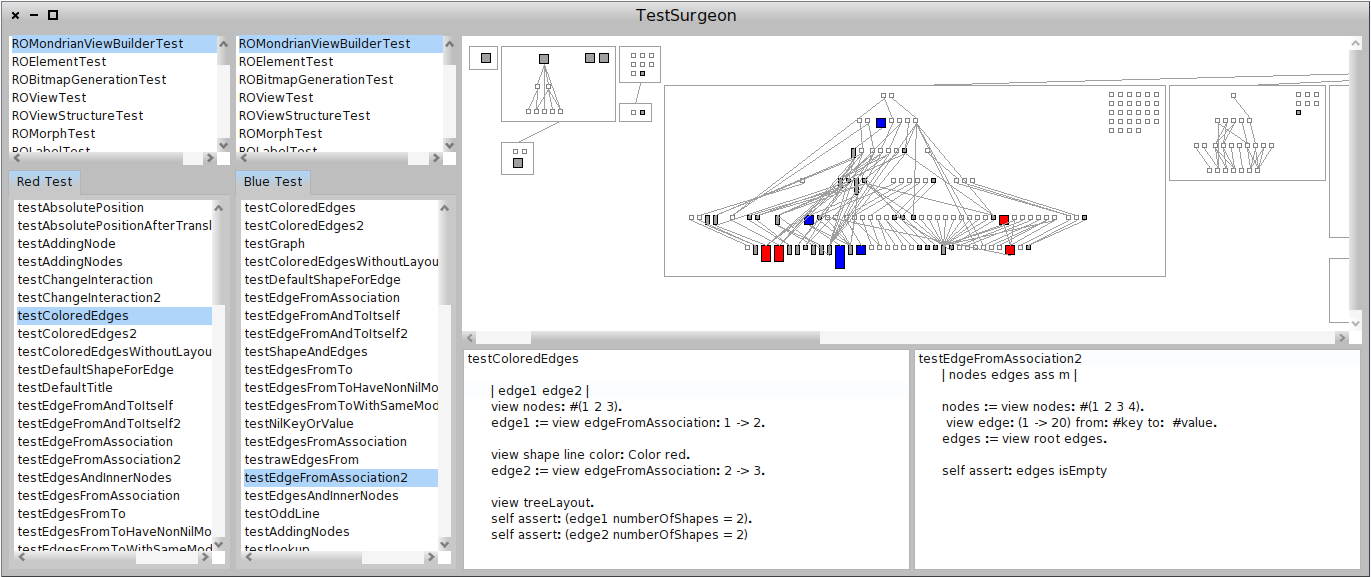
\includegraphics[scale=0.35]{screenshot_ts.png}
	\caption{Captura de pantalla de la versión actual de TestSurgeon}	
\end{figure}
\vspace*{0.7 cm}

\par TestSurgeon provee una visualización enfocada en diferencias entre la ejecución de dos tests sobre el código testeado. Pharo es un lenguaje que se rige por el pardigma de Programación Orientada a Objetos por lo cual los elementos básicos que describen cualquier software son las métodos y las clases. Es por eso que en la visualización estos elementos son parte fundamental, tal como se ve en la figura \ref{blueprint-cls-mtds}. Las cajas grandes representan clases testeadas y las eventuales lineas entre ellos grafica la jerarquía de clases. Ahora, dentro de cada clase se pueden apreciar cuadrados más pequeños que reprensentan sus métodos. Estos métodos pueden ser de 4 colores distintos:

\begin{itemize}
\item Rojo: el método fue llamado solo por el test rojo durante la ejecución
\item Azul: el método fue llamado solo por el test azul durante la ejecución
\item Gris: el método fue llamado los dos tests
\item Blanco: el método no fue llamado durante la ejecucion de ninguno de los tests
\end{itemize}

Las líneas entre métodos representan llamadas internas (invocaciones a \emph{self} en Pharo, el equivalente a \emph{this} de Java) de un método a otro.

\begin{figure}[h!]
	\centering
    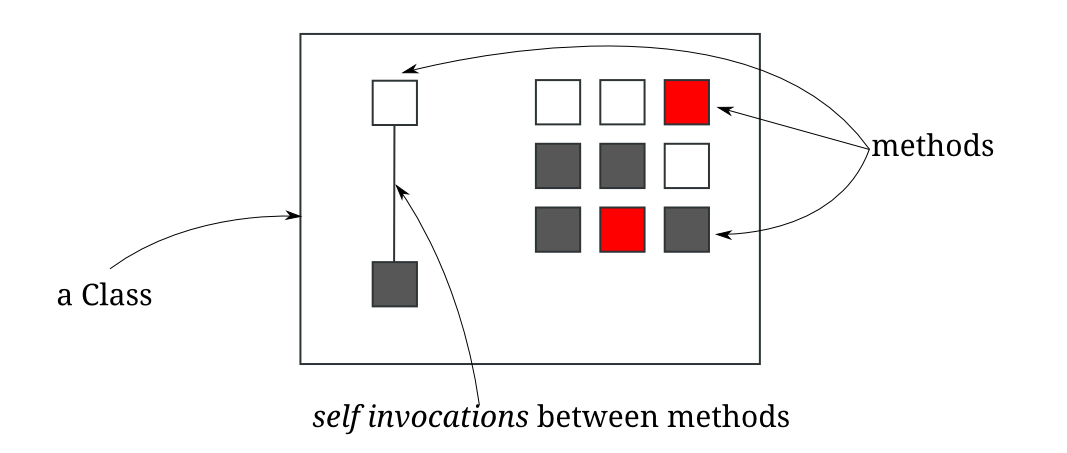
\includegraphics[scale=0.4]{cls_mtds.png}
	\caption{Visualización de una clase y sus métodos en TestSurgeon}	
		\label{blueprint-cls-mtds}
\end{figure}

\par La comparación se realiza obsevando la forma de los métodos. 
En particular la altura de un método representa la cantidad de veces que se llamó a dicho método durante la ejecución de los tests. 
El ancho, por su parte, está relacionado a la cantidad de distintos objetos que recibieron dicho método como mensaje durante la ejecución de cada test. 
El alto y el ancho representan  entre métricas para cada ejecucion de test. 
Esta información se visualiza en función de su \emph{diferencias} (o \emph{deltas}) entre las métricas. Por ende, entre más grande se vea un método mayor fue la diferencia entre las métricas antes mencionadas para ese método como se puede ver en forma resumida en la figura \ref{blueprint-summary}. \\

\par Entonces, dos métodos van a ser similares entre más pequeños sean sus métodos y cuanto más métodos de color gris hayan. Por el contrario, si se perciben métodos grandes y rojos o azules, entonces hay cierta predominancia de uno de los dos tests por las intancias de dicha clase.

\begin{figure}[h!]
	\centering
    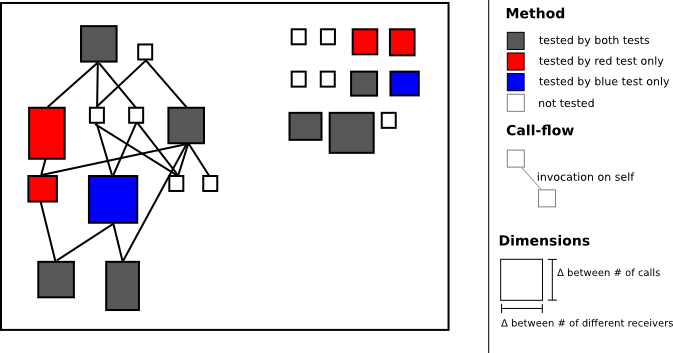
\includegraphics[scale=0.6]{blueprint-summary.png}
	\caption{Resumen de la visualización de TestSurgeon}
	\label{blueprint-summary}	
\end{figure}

\par TestSurgeon fue presentado en la International Conference on Software Engineering[\ref{restruct-utests}] (ICSE 2012, principal conferencia en el área, L0) donde compitió en la ACM Student Research Competition obteniendo el primer lugar en la categoría de pregrado\footnote{SRC Winners, \url{http://src.acm.org/winners.html}}.

\par Si bien TestSurgeon es un buen inicio, es difícil aplicarlo para usos cotidianos de un desarrollador o miembro del equipo de Aseguramiento de Calidad(QA). Esto porque cuando la cantidad de métodos de test es grande, la comparación 1 a 1 se hace tediosa. Por lo cual el siguiente paso es visualizar diferencias entre \textbf{grupos de métodos de tests} para encontrar grupos afines y que representen una estructura mejor para los casos de prueba.

\par Por otro lado, aspectos de performance que se ven involucrados en las refactorizaciones propuestas no se están midiendo. Otro aspecto interesante es ver la diferencia entre las coberturas de las distintas versiones de tests: pre y post refactorización. Aun cuando estas preguntas son interesantes y estarán consideradas durante el desarrollo de TestSurgeon, el alcance de este trabajo no abarca esos problemas en detalle.	


%%%%%%%%%%%%%%%%%%%%%%%%%%%%%%%%%%%%%%%%%%%%%
% OBJETIVOS
%%%%%%%%%%%%%%%%%%%%%%%%%%%%%%%%%%%%%%%%%%%%%

% Cual es el problema?
% Pq es importante, relevante e interesante?
% Como se resuelve actualmente?

\section{Objetivos}
\par El objetivo general de este trabajo es crear una herramienta que permita a los desarrolladores refactorizar y reestructurar sus test de una manera más fácil y mejorar la performance de estos.

\subsection*{Objetivos Específicos}
\begin{itemize}
\item Identificación de las métricas relevantes para caracterización de tests methods desde el punto de vista de un análisis dinámico
\item Desarrollar una visualización que permita detectar redundancia y solapamiento entre grupos de test methods (o unit tests)
\item Investigar refactorizaciones automáticas y semi-automáticas para unit tests y sus implicancias en performance y cobertura
\item Desarrollar una interfaz gráfica efectiva y usable para el uso cotidiano dentro del desarrollo de software
\end{itemize}


%%%%%%%%%%%%%%%%%%%%%%%%%%%%%%%%%%%%%%%%%%%%%
% METODOLOGIA
%%%%%%%%%%%%%%%%%%%%%%%%%%%%%%%%%%%%%%%%%%%%%

\section{Metodología}
\par Dado lo innovador del proyecto, se prevee una metodologia de desarrollo iterativa de pequeños experimentos que puedan ser rápidamente implementados y validados.
\par Para su realización, validación y retroalimentación, se coordinarán esfuerzos con los siguientes proyectos:
\begin{itemize}
\item \textbf{Spec}:  Framework de intefaz gráfica de usuario, desarollado por el grupo de investigacion RMoD en INRIA Lille Nord Europe. \url{http://rmod.lille.inria.fr}
\item \textbf{Glamour}: Framework para desarrollar browsers de navegación. Glamour es mantenido y desarrollado en la Universidad de Bern y NetStyle.ch, en Suiza. \url{http://moosetechnology.org/tools/glamour}
\item \textbf{Moose}: Moose es una plataforma para analizar software. Moose es el resultado de un consorcio entre universidades europeas y sudamericanas. \url{http://moosetechnology.org}
\item \textbf{MediaGeniX}: Compañia Belga que produce software para grandes cadenas de TV.
\end{itemize}

\par Cada uno de esos cuatro proyectos han expresado la necesidad de mejorar y restructurar su set de Unit Tests.

\par Sin embargo, la primera gran característica a desarrollar será la visualización de diferencias entre \emph{grupos de tests}. Esto pensando en encontrar grupos de tests que representen de mejor manera un caso de prueba y que además cuenten con mejor performance.


%%%%%%%%%%%%%%%%%%%%%%%%%%%%%%%%%%%%%%%%%%%%%
% CRONOGRAMA
%%%%%%%%%%%%%%%%%%%%%%%%%%%%%%%%%%%%%%%%%%%%%

\section{Cronograma}
\par Para este proyecto, se definen dos fases: desarrollo de la herramienta y escritura del documento de memoria.  
\begin{itemize}
	\item \textbf{Desarrollo de la Herramienta (5 meses)} Si bien los objetivos están definidos, el desarrollo es exploratorio y necesita constante validación. 
		\begin{enumerate}
			\item \textbf{Definición y diseño del features (0.5 semana)} En esta fase se define y diseña el siguiente feature.
			\item \textbf{Implementación (1.5 semanas)} Se implementa el feature definido. 
			\item \textbf{Experimentación con la versión actual de TestSurgeon (2 semanas)} En esta fase se obtiene retroalimentación sobre la efectividad de los cambios en la visualización e identificación de escenarios de refactoring.
		\end{enumerate}
	\item \textbf{Escritura del documento de la memoria (1 mes):} Finalmente se destinará tiempo para documentar TestSurgeon y escribir el documento de memoria. Esto sin perjuicio de que el documento se escriba en paralelo al desarrollo de la herramienta.
\end{itemize}

\vspace*{0.5cm}

\begin{figure}[h!]
	\centering
    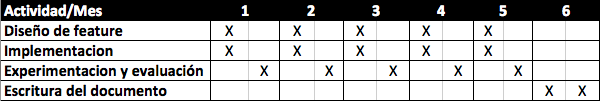
\includegraphics[scale=0.8]{carta_gantt.png}
	\caption{Carta Gantt de planificación}	
		\label{blueprint-cls-mtds}
\end{figure}

\newpage
\section{Referencias Bibliográficas}
\begin{enumerate}
	\item Martin Fowler. \emph{Continuous Integration} - \url{http://www.martinfowler.com/articles/continuousIntegration.html} - \emph{Última revisión: 14 de septiembre, 2012}. \label{contint}

	\item Robert Cecil Martin. \emph{Agile Software Development. Principles, Patterns, and Practices}. Prentice-Hall, 2002.\label{unclebob}

	\item Kent Beck. \emph{Test Driven Development: By Example}. Addison-Wesley Longman, 2002.\label{tdd-beck}

	\item Fowler, Martin y Highsmith, Jim. \emph{The Agile Manifesto}, Software Development Magazine, 2002. \url{http://agilemanifesto.org} - \emph{Última revisión: 14 de septiembre, 2012}.\label{agilemanifiesto}

	\item Alexandre Bergel and Felipe Ba\~nados and Romain Robbes and David R\"othlisberger, Spy: A flexible Code Profiling Framework. \emph{Journal of Computer Languages, Systems and Structures}, December 2011. \url{http://bergel.eu/download/papers/Berg10f-Spy.pdf} - \emph{Última revisión: 14 de septiembre, 2012}.\label{spy-framework}

	\item Pablo Estefó. Restructuring Unit Test with TestSurgeon. \emph{Proceedings of International Conference on Software Engineering(ICSE) 2012 }. \label{restruct-utests}

	\item Michele Lanza y Stéphane Ducasse. Polymetric views—a lightweight visual approach to reverse engineering. \emph{Transactions on Software Engineering (TSE)}, September 2003. \label{polimetric-views}

\end{enumerate}

\end{document}
